\begin{figure}[htbp]
\centering
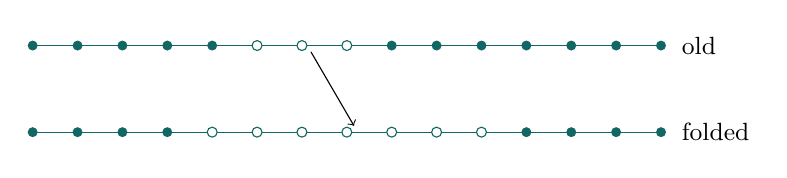
\begin{tikzpicture}[x=.57cm,y=1cm,font=\small]
  \definecolor{lamp}{RGB}{18,102,99}
  \foreach \y/\first/\last/\name in {1.1/5/7/old,0/4/10/folded} {
    \draw[lamp] (0,\y) -- (14,\y) node[right=4pt,text=black] {\name};
    \foreach \x in {0,...,14} {
      \ifnum\x<\first \fill[lamp] (\x,\y) circle (1.8pt);
      \else\ifnum\x>\last \fill[lamp] (\x,\y) circle (1.8pt);
      \else \draw[lamp,fill=white] (\x,\y) circle (1.8pt);
      \fi\fi
    }
  }
  \draw[->] (6.2,1.02) -- (7.16,.08);
\end{tikzpicture}
\caption{One cycle, cut open. White lamps are forgotten. When making a new site at a nearby
height we can inherit all specified lamps by increasing the radius by a constant. Only boundedly
many old site labels per height can compete to feed one such label.}
\label{fig:window}
\end{figure}
